% REV01 Thu 24 Jun 2021 05:29:02 WIB
% START Tue 04 May 2021 13:55:16 WIB

\chapter{THE WHOLE CASE SO FAR}

Bradley Headstone held fast by that other interview he was to have with
Lizzie Hexam. In stipulating for it, he had been impelled by a feeling
little short of desperation, and the feeling abided by him. It was very
soon after his interview with the Secretary, that he and Charley Hexam
set out one leaden evening, not unnoticed by Miss Peecher, to have this
desperate interview accomplished.

‘That dolls’ dressmaker,’ said Bradley, ‘is favourable neither to me nor
to you, Hexam.’

‘A pert crooked little chit, Mr Headstone! I knew she would put herself
in the way, if she could, and would be sure to strike in with something
impertinent. It was on that account that I proposed our going to the
City to-night and meeting my sister.’

‘So I supposed,’ said Bradley, getting his gloves on his nervous hands
as he walked. ‘So I supposed.’

‘Nobody but my sister,’ pursued Charley, ‘would have found out such an
extraordinary companion. She has done it in a ridiculous fancy of giving
herself up to another. She told me so, that night when we went there.’

‘Why should she give herself up to the dressmaker?’ asked Bradley.

‘Oh!’ said the boy, colouring. ‘One of her romantic ideas! I tried to
convince her so, but I didn’t succeed. However, what we have got to do,
is, to succeed to-night, Mr Headstone, and then all the rest follows.’

‘You are still sanguine, Hexam.’

‘Certainly I am, sir. Why, we have everything on our side.’

‘Except your sister, perhaps,’ thought Bradley. But he only gloomily
thought it, and said nothing.

‘Everything on our side,’ repeated the boy with boyish confidence.
‘Respectability, an excellent connexion for me, common sense,
everything!’

‘To be sure, your sister has always shown herself a devoted sister,’
said Bradley, willing to sustain himself on even that low ground of
hope.

‘Naturally, Mr Headstone, I have a good deal of influence with her.
And now that you have honoured me with your confidence and spoken to me
first, I say again, we have everything on our side.’

And Bradley thought again, ‘Except your sister, perhaps.’

A grey dusty withered evening in London city has not a hopeful aspect.
The closed warehouses and offices have an air of death about them, and
the national dread of colour has an air of mourning. The towers and
steeples of the many house-encompassed churches, dark and dingy as the
sky that seems descending on them, are no relief to the general gloom;
a sun-dial on a church-wall has the look, in its useless black shade, of
having failed in its business enterprise and stopped payment for ever;
melancholy waifs and strays of housekeepers and porter sweep melancholy
waifs and strays of papers and pins into the kennels, and other more
melancholy waifs and strays explore them, searching and stooping and
poking for anything to sell. The set of humanity outward from the City
is as a set of prisoners departing from gaol, and dismal Newgate
seems quite as fit a stronghold for the mighty Lord Mayor as his own
state-dwelling.

On such an evening, when the city grit gets into the hair and eyes and
skin, and when the fallen leaves of the few unhappy city trees grind
down in corners under wheels of wind, the schoolmaster and the pupil
emerged upon the Leadenhall Street region, spying eastward for Lizzie.
Being something too soon in their arrival, they lurked at a corner,
waiting for her to appear. The best-looking among us will not look very
well, lurking at a corner, and Bradley came out of that disadvantage
very poorly indeed.

‘Here she comes, Mr Headstone! Let us go forward and meet her.’

As they advanced, she saw them coming, and seemed rather troubled. But
she greeted her brother with the usual warmth, and touched the extended
hand of Bradley.

‘Why, where are you going, Charley, dear?’ she asked him then.

‘Nowhere. We came on purpose to meet you.’

‘To meet me, Charley?’

‘Yes. We are going to walk with you. But don’t let us take the great
leading streets where every one walks, and we can’t hear ourselves
speak. Let us go by the quiet backways. Here’s a large paved court by
this church, and quiet, too. Let us go up here.’

‘But it’s not in the way, Charley.’

‘Yes it is,’ said the boy, petulantly. ‘It’s in my way, and my way is
yours.’

She had not released his hand, and, still holding it, looked at him with
a kind of appeal. He avoided her eyes, under pretence of saying, ‘Come
along, Mr Headstone.’ Bradley walked at his side--not at hers--and the
brother and sister walked hand in hand. The court brought them to a
churchyard; a paved square court, with a raised bank of earth about
breast high, in the middle, enclosed by iron rails. Here, conveniently
and healthfully elevated above the level of the living, were the dead,
and the tombstones; some of the latter droopingly inclined from the
perpendicular, as if they were ashamed of the lies they told.

They paced the whole of this place once, in a constrained and
uncomfortable manner, when the boy stopped and said:

‘Lizzie, Mr Headstone has something to say to you. I don’t wish to be an
interruption either to him or to you, and so I’ll go and take a little
stroll and come back. I know in a general way what Mr Headstone intends
to say, and I very highly approve of it, as I hope--and indeed I do
not doubt--you will. I needn’t tell you, Lizzie, that I am under great
obligations to Mr Headstone, and that I am very anxious for Mr Headstone
to succeed in all he undertakes. As I hope--and as, indeed, I don’t
doubt--you must be.’

‘Charley,’ returned his sister, detaining his hand as he withdrew it, ‘I
think you had better stay. I think Mr Headstone had better not say what
he thinks of saying.’

‘Why, how do you know what it is?’ returned the boy.

‘Perhaps I don’t, but--’

‘Perhaps you don’t? No, Liz, I should think not. If you knew what
it was, you would give me a very different answer. There; let go; be
sensible. I wonder you don’t remember that Mr Headstone is looking on.’

She allowed him to separate himself from her, and he, after saying, ‘Now
Liz, be a rational girl and a good sister,’ walked away. She remained
standing alone with Bradley Headstone, and it was not until she raised
her eyes, that he spoke.

‘I said,’ he began, ‘when I saw you last, that there was something
unexplained, which might perhaps influence you. I have come this evening
to explain it. I hope you will not judge of me by my hesitating manner
when I speak to you. You see me at my greatest disadvantage. It is most
unfortunate for me that I wish you to see me at my best, and that I know
you see me at my worst.’

She moved slowly on when he paused, and he moved slowly on beside her.

‘It seems egotistical to begin by saying so much about myself,’ he
resumed, ‘but whatever I say to you seems, even in my own ears, below
what I want to say, and different from what I want to say. I can’t help
it. So it is. You are the ruin of me.’

She started at the passionate sound of the last words, and at the
passionate action of his hands, with which they were accompanied.

‘Yes! you are the ruin--the ruin--the ruin--of me. I have no resources
in myself, I have no confidence in myself, I have no government of
myself when you are near me or in my thoughts. And you are always in my
thoughts now. I have never been quit of you since I first saw you. Oh,
that was a wretched day for me! That was a wretched, miserable day!’

A touch of pity for him mingled with her dislike of him, and she said:
‘Mr Headstone, I am grieved to have done you any harm, but I have never
meant it.’

‘There!’ he cried, despairingly. ‘Now, I seem to have reproached you,
instead of revealing to you the state of my own mind! Bear with me. I am
always wrong when you are in question. It is my doom.’

Struggling with himself, and by times looking up at the deserted windows
of the houses as if there could be anything written in their grimy panes
that would help him, he paced the whole pavement at her side, before he
spoke again.

‘I must try to give expression to what is in my mind; it shall and must
be spoken. Though you see me so confounded--though you strike me so
helpless--I ask you to believe that there are many people who think well
of me; that there are some people who highly esteem me; that I have in
my way won a Station which is considered worth winning.’

‘Surely, Mr Headstone, I do believe it. Surely I have always known it
from Charley.’

‘I ask you to believe that if I were to offer my home such as it is, my
station such as it is, my affections such as they are, to any one of the
best considered, and best qualified, and most distinguished, among the
young women engaged in my calling, they would probably be accepted. Even
readily accepted.’

‘I do not doubt it,’ said Lizzie, with her eyes upon the ground.

‘I have sometimes had it in my thoughts to make that offer and to settle
down as many men of my class do: I on the one side of a school, my wife
on the other, both of us interested in the same work.’

‘Why have you not done so?’ asked Lizzie Hexam. ‘Why do you not do so?’

‘Far better that I never did! The only one grain of comfort I have had
these many weeks,’ he said, always speaking passionately, and, when
most emphatic, repeating that former action of his hands, which was
like flinging his heart’s blood down before her in drops upon the
pavement-stones; ‘the only one grain of comfort I have had these many
weeks is, that I never did. For if I had, and if the same spell had come
upon me for my ruin, I know I should have broken that tie asunder as if
it had been thread.’

She glanced at him with a glance of fear, and a shrinking gesture. He
answered, as if she had spoken.

‘No! It would not have been voluntary on my part, any more than it is
voluntary in me to be here now. You draw me to you. If I were shut up in
a strong prison, you would draw me out. I should break through the wall
to come to you. If I were lying on a sick bed, you would draw me up--to
stagger to your feet and fall there.’

The wild energy of the man, now quite let loose, was absolutely
terrible. He stopped and laid his hand upon a piece of the coping of the
burial-ground enclosure, as if he would have dislodged the stone.

‘No man knows till the time comes, what depths are within him. To some
men it never comes; let them rest and be thankful! To me, you brought
it; on me, you forced it; and the bottom of this raging sea,’ striking
himself upon the breast, ‘has been heaved up ever since.’

‘Mr Headstone, I have heard enough. Let me stop you here. It will be
better for you and better for me. Let us find my brother.’

‘Not yet. It shall and must be spoken. I have been in torments ever
since I stopped short of it before. You are alarmed. It is another of my
miseries that I cannot speak to you or speak of you without stumbling at
every syllable, unless I let the check go altogether and run mad. Here
is a man lighting the lamps. He will be gone directly. I entreat of you
let us walk round this place again. You have no reason to look alarmed;
I can restrain myself, and I will.’

She yielded to the entreaty--how could she do otherwise!--and they paced
the stones in silence. One by one the lights leaped up making the cold
grey church tower more remote, and they were alone again. He said no
more until they had regained the spot where he had broken off; there, he
again stood still, and again grasped the stone. In saying what he said
then, he never looked at her; but looked at it and wrenched at it.

‘You know what I am going to say. I love you. What other men may mean
when they use that expression, I cannot tell; what I mean is, that I am
under the influence of some tremendous attraction which I have resisted
in vain, and which overmasters me. You could draw me to fire, you could
draw me to water, you could draw me to the gallows, you could draw me to
any death, you could draw me to anything I have most avoided, you could
draw me to any exposure and disgrace. This and the confusion of my
thoughts, so that I am fit for nothing, is what I mean by your being the
ruin of me. But if you would return a favourable answer to my offer
of myself in marriage, you could draw me to any good--every good--with
equal force. My circumstances are quite easy, and you would want for
nothing. My reputation stands quite high, and would be a shield for
yours. If you saw me at my work, able to do it well and respected in
it, you might even come to take a sort of pride in me;--I would try hard
that you should. Whatever considerations I may have thought of against
this offer, I have conquered, and I make it with all my heart. Your
brother favours me to the utmost, and it is likely that we might live
and work together; anyhow, it is certain that he would have my best
influence and support. I don’t know what I could say more if I tried. I
might only weaken what is ill enough said as it is. I only add that
if it is any claim on you to be in earnest, I am in thorough earnest,
dreadful earnest.’

The powdered mortar from under the stone at which he wrenched, rattled
on the pavement to confirm his words.

‘Mr Headstone--’

‘Stop! I implore you, before you answer me, to walk round this place
once more. It will give you a minute’s time to think, and me a minute’s
time to get some fortitude together.’

Again she yielded to the entreaty, and again they came back to the same
place, and again he worked at the stone.

‘Is it,’ he said, with his attention apparently engrossed by it, ‘yes,
or no?’

‘Mr Headstone, I thank you sincerely, I thank you gratefully, and hope
you may find a worthy wife before long and be very happy. But it is no.’

‘Is no short time necessary for reflection; no weeks or days?’ he asked,
in the same half-suffocated way.

‘None whatever.’

‘Are you quite decided, and is there no chance of any change in my
favour?’

‘I am quite decided, Mr Headstone, and I am bound to answer I am certain
there is none.’

‘Then,’ said he, suddenly changing his tone and turning to her, and
bringing his clenched hand down upon the stone with a force that laid
the knuckles raw and bleeding; ‘then I hope that I may never kill him!’

The dark look of hatred and revenge with which the words broke from his
livid lips, and with which he stood holding out his smeared hand as
if it held some weapon and had just struck a mortal blow, made her so
afraid of him that she turned to run away. But he caught her by the arm.

‘Mr Headstone, let me go. Mr Headstone, I must call for help!’

‘It is I who should call for help,’ he said; ‘you don’t know yet how
much I need it.’

The working of his face as she shrank from it, glancing round for her
brother and uncertain what to do, might have extorted a cry from her in
another instant; but all at once he sternly stopped it and fixed it, as
if Death itself had done so.

‘There! You see I have recovered myself. Hear me out.’

With much of the dignity of courage, as she recalled her self-reliant
life and her right to be free from accountability to this man, she
released her arm from his grasp and stood looking full at him. She had
never been so handsome, in his eyes. A shade came over them while
he looked back at her, as if she drew the very light out of them to
herself.

‘This time, at least, I will leave nothing unsaid,’ he went on, folding
his hands before him, clearly to prevent his being betrayed into any
impetuous gesture; ‘this last time at least I will not be tortured with
after-thoughts of a lost opportunity. Mr Eugene Wrayburn.’

‘Was it of him you spoke in your ungovernable rage and violence?’ Lizzie
Hexam demanded with spirit.

He bit his lip, and looked at her, and said never a word.

‘Was it Mr Wrayburn that you threatened?’

He bit his lip again, and looked at her, and said never a word.

‘You asked me to hear you out, and you will not speak. Let me find my
brother.’

‘Stay! I threatened no one.’

Her look dropped for an instant to his bleeding hand. He lifted it to
his mouth, wiped it on his sleeve, and again folded it over the other.
‘Mr Eugene Wrayburn,’ he repeated.

‘Why do you mention that name again and again, Mr Headstone?’

‘Because it is the text of the little I have left to say. Observe! There
are no threats in it. If I utter a threat, stop me, and fasten it upon
me. Mr Eugene Wrayburn.’

A worse threat than was conveyed in his manner of uttering the name,
could hardly have escaped him.

‘He haunts you. You accept favours from him. You are willing enough to
listen to HIM. I know it, as well as he does.’

‘Mr Wrayburn has been considerate and good to me, sir,’ said Lizzie,
proudly, ‘in connexion with the death and with the memory of my poor
father.’

‘No doubt. He is of course a very considerate and a very good man, Mr
Eugene Wrayburn.’

‘He is nothing to you, I think,’ said Lizzie, with an indignation she
could not repress.

‘Oh yes, he is. There you mistake. He is much to me.’

‘What can he be to you?’

‘He can be a rival to me among other things,’ said Bradley.

‘Mr Headstone,’ returned Lizzie, with a burning face, ‘it is cowardly in
you to speak to me in this way. But it makes me able to tell you that
I do not like you, and that I never have liked you from the first, and
that no other living creature has anything to do with the effect you
have produced upon me for yourself.’

His head bent for a moment, as if under a weight, and he then looked up
again, moistening his lips. ‘I was going on with the little I had left
to say. I knew all this about Mr Eugene Wrayburn, all the while you were
drawing me to you. I strove against the knowledge, but quite in vain. It
made no difference in me. With Mr Eugene Wrayburn in my mind, I went
on. With Mr Eugene Wrayburn in my mind, I spoke to you just now. With Mr
Eugene Wrayburn in my mind, I have been set aside and I have been cast
out.’

‘If you give those names to my thanking you for your proposal
and declining it, is it my fault, Mr Headstone?’ said Lizzie,
compassionating the bitter struggle he could not conceal, almost as much
as she was repelled and alarmed by it.

‘I am not complaining,’ he returned, ‘I am only stating the case. I had
to wrestle with my self-respect when I submitted to be drawn to you in
spite of Mr Wrayburn. You may imagine how low my self-respect lies now.’

She was hurt and angry; but repressed herself in consideration of his
suffering, and of his being her brother’s friend.

‘And it lies under his feet,’ said Bradley, unfolding his hands in spite
of himself, and fiercely motioning with them both towards the stones of
the pavement. ‘Remember that! It lies under that fellow’s feet, and he
treads upon it and exults above it.’

‘He does not!’ said Lizzie.

‘He does!’ said Bradley. ‘I have stood before him face to face, and he
crushed me down in the dirt of his contempt, and walked over me. Why?
Because he knew with triumph what was in store for me to-night.’

‘O, Mr Headstone, you talk quite wildly.’

‘Quite collectedly. I know what I say too well. Now I have said all. I
have used no threat, remember; I have done no more than show you how the
case stands;--how the case stands, so far.’

At this moment her brother sauntered into view close by. She darted to
him, and caught him by the hand. Bradley followed, and laid his heavy
hand on the boy’s opposite shoulder.

‘Charley Hexam, I am going home. I must walk home by myself to-night,
and get shut up in my room without being spoken to. Give me half an
hour’s start, and let me be, till you find me at my work in the morning.
I shall be at my work in the morning just as usual.’

Clasping his hands, he uttered a short unearthly broken cry, and went
his way. The brother and sister were left looking at one another near
a lamp in the solitary churchyard, and the boy’s face clouded and
darkened, as he said in a rough tone: ‘What is the meaning of this? What
have you done to my best friend? Out with the truth!’

‘Charley!’ said his sister. ‘Speak a little more considerately!’

‘I am not in the humour for consideration, or for nonsense of any sort,’
replied the boy. ‘What have you been doing? Why has Mr Headstone gone
from us in that way?’

‘He asked me--you know he asked me--to be his wife, Charley.’

‘Well?’ said the boy, impatiently.

‘And I was obliged to tell him that I could not be his wife.’

‘You were obliged to tell him,’ repeated the boy angrily, between his
teeth, and rudely pushing her away. ‘You were obliged to tell him! Do
you know that he is worth fifty of you?’

‘It may easily be so, Charley, but I cannot marry him.’

‘You mean that you are conscious that you can’t appreciate him, and
don’t deserve him, I suppose?’

‘I mean that I do not like him, Charley, and that I will never marry
him.’

‘Upon my soul,’ exclaimed the boy, ‘you are a nice picture of a sister!
Upon my soul, you are a pretty piece of disinterestedness! And so all my
endeavours to cancel the past and to raise myself in the world, and to
raise you with me, are to be beaten down by YOUR low whims; are they?’

‘I will not reproach you, Charley.’

‘Hear her!’ exclaimed the boy, looking round at the darkness. ‘She won’t
reproach me! She does her best to destroy my fortunes and her own,
and she won’t reproach me! Why, you’ll tell me, next, that you won’t
reproach Mr Headstone for coming out of the sphere to which he is an
ornament, and putting himself at YOUR feet, to be rejected by YOU!’

‘No, Charley; I will only tell you, as I told himself, that I thank him
for doing so, that I am sorry he did so, and that I hope he will do much
better, and be happy.’

Some touch of compunction smote the boy’s hardening heart as he looked
upon her, his patient little nurse in infancy, his patient friend,
adviser, and reclaimer in boyhood, the self-forgetting sister who had
done everything for him. His tone relented, and he drew her arm through
his.

‘Now, come, Liz; don’t let us quarrel: let us be reasonable and talk
this over like brother and sister. Will you listen to me?’

‘Oh, Charley!’ she replied through her starting tears; ‘do I not listen
to you, and hear many hard things!’

‘Then I am sorry. There, Liz! I am unfeignedly sorry. Only you do put me
out so. Now see. Mr Headstone is perfectly devoted to you. He has told
me in the strongest manner that he has never been his old self for one
single minute since I first brought him to see you. Miss Peecher, our
schoolmistress--pretty and young, and all that--is known to be very much
attached to him, and he won’t so much as look at her or hear of her.
Now, his devotion to you must be a disinterested one; mustn’t it? If he
married Miss Peecher, he would be a great deal better off in all worldly
respects, than in marrying you. Well then; he has nothing to get by it,
has he?’

‘Nothing, Heaven knows!’

‘Very well then,’ said the boy; ‘that’s something in his favour, and a
great thing. Then I come in. Mr Headstone has always got me on, and he
has a good deal in his power, and of course if he was my brother-in-law
he wouldn’t get me on less, but would get me on more. Mr Headstone
comes and confides in me, in a very delicate way, and says, “I hope my
marrying your sister would be agreeable to you, Hexam, and useful to
you?” I say, “There’s nothing in the world, Mr Headstone, that I could
be better pleased with.” Mr Headstone says, “Then I may rely upon your
intimate knowledge of me for your good word with your sister, Hexam?”
 And I say, “Certainly, Mr Headstone, and naturally I have a good deal of
influence with her.” So I have; haven’t I, Liz?’

‘Yes, Charley.’

‘Well said! Now, you see, we begin to get on, the moment we begin to
be really talking it over, like brother and sister. Very well. Then
YOU come in. As Mr Headstone’s wife you would be occupying a most
respectable station, and you would be holding a far better place in
society than you hold now, and you would at length get quit of the
river-side and the old disagreeables belonging to it, and you would be
rid for good of dolls’ dressmakers and their drunken fathers, and the
like of that. Not that I want to disparage Miss Jenny Wren: I dare
say she is all very well in her way; but her way is not your way as
Mr Headstone’s wife. Now, you see, Liz, on all three accounts--on
Mr Headstone’s, on mine, on yours--nothing could be better or more
desirable.’

They were walking slowly as the boy spoke, and here he stood still, to
see what effect he had made. His sister’s eyes were fixed upon him; but
as they showed no yielding, and as she remained silent, he walked her on
again. There was some discomfiture in his tone as he resumed, though he
tried to conceal it.

‘Having so much influence with you, Liz, as I have, perhaps I should
have done better to have had a little chat with you in the first
instance, before Mr Headstone spoke for himself. But really all this in
his favour seemed so plain and undeniable, and I knew you to have always
been so reasonable and sensible, that I didn’t consider it worth while.
Very likely that was a mistake of mine. However, it’s soon set right.
All that need be done to set it right, is for you to tell me at once
that I may go home and tell Mr Headstone that what has taken place is
not final, and that it will all come round by-and-by.’

He stopped again. The pale face looked anxiously and lovingly at him,
but she shook her head.

‘Can’t you speak?’ said the boy sharply.

‘I am very unwilling to speak, Charley. If I must, I must. I cannot
authorize you to say any such thing to Mr Headstone: I cannot allow you
to say any such thing to Mr Headstone. Nothing remains to be said to him
from me, after what I have said for good and all, to-night.’

‘And this girl,’ cried the boy, contemptuously throwing her off again,
‘calls herself a sister!’

‘Charley, dear, that is the second time that you have almost struck
me. Don’t be hurt by my words. I don’t mean--Heaven forbid!--that you
intended it; but you hardly know with what a sudden swing you removed
yourself from me.’

‘However!’ said the boy, taking no heed of the remonstrance, and
pursuing his own mortified disappointment, ‘I know what this means, and
you shall not disgrace me.’

‘It means what I have told you, Charley, and nothing more.’

‘That’s not true,’ said the boy in a violent tone, ‘and you know it’s
not. It means your precious Mr Wrayburn; that’s what it means.’

‘Charley! If you remember any old days of ours together, forbear!’

‘But you shall not disgrace me,’ doggedly pursued the boy. ‘I am
determined that after I have climbed up out of the mire, you shall not
pull me down. You can’t disgrace me if I have nothing to do with you,
and I will have nothing to do with you for the future.’

‘Charley! On many a night like this, and many a worse night, I have sat
on the stones of the street, hushing you in my arms. Unsay those words
without even saying you are sorry for them, and my arms are open to you
still, and so is my heart.’

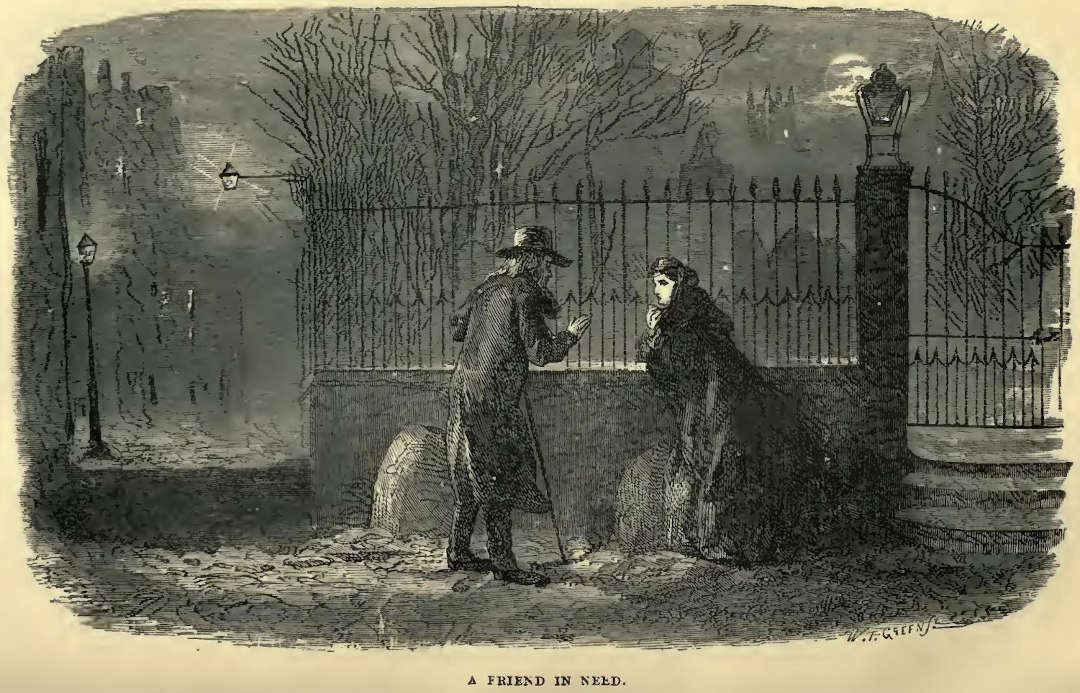
\includegraphics[scale=2.3]{02-15-01}

‘I’ll not unsay them. I’ll say them again. You are an inveterately bad
girl, and a false sister, and I have done with you. For ever, I have
done with you!’

He threw up his ungrateful and ungracious hand as if it set up a barrier
between them, and flung himself upon his heel and left her. She remained
impassive on the same spot, silent and motionless, until the striking
of the church clock roused her, and she turned away. But then, with the
breaking up of her immobility came the breaking up of the waters that
the cold heart of the selfish boy had frozen. And ‘O that I were lying
here with the dead!’ and ‘O Charley, Charley, that this should be the
end of our pictures in the fire!’ were all the words she said, as she
laid her face in her hands on the stone coping.

A figure passed by, and passed on, but stopped and looked round at
her. It was the figure of an old man with a bowed head, wearing a large
brimmed low-crowned hat, and a long-skirted coat. After hesitating a
little, the figure turned back, and, advancing with an air of gentleness
and compassion, said:

‘Pardon me, young woman, for speaking to you, but you are under some
distress of mind. I cannot pass upon my way and leave you weeping here
alone, as if there was nothing in the place. Can I help you? Can I do
anything to give you comfort?’

She raised her head at the sound of these kind words, and answered
gladly, ‘O, Mr Riah, is it you?’

‘My daughter,’ said the old man, ‘I stand amazed! I spoke as to a
stranger. Take my arm, take my arm. What grieves you? Who has done this?
Poor girl, poor girl!’

‘My brother has quarrelled with me,’ sobbed Lizzie, ‘and renounced me.’

‘He is a thankless dog,’ said the Jew, angrily. ‘Let him go. Shake the
dust from thy feet and let him go. Come, daughter! Come home with me--it
is but across the road--and take a little time to recover your peace and
to make your eyes seemly, and then I will bear you company through the
streets. For it is past your usual time, and will soon be late, and the
way is long, and there is much company out of doors to-night.’

She accepted the support he offered her, and they slowly passed out
of the churchyard. They were in the act of emerging into the main
thoroughfare, when another figure loitering discontentedly by, and
looking up the street and down it, and all about, started and exclaimed,
‘Lizzie! why, where have you been? Why, what’s the matter?’

As Eugene Wrayburn thus addressed her, she drew closer to the Jew, and
bent her head. The Jew having taken in the whole of Eugene at one sharp
glance, cast his eyes upon the ground, and stood mute.

‘Lizzie, what is the matter?’

‘Mr Wrayburn, I cannot tell you now. I cannot tell you to-night, if I
ever can tell you. Pray leave me.’

‘But, Lizzie, I came expressly to join you. I came to walk home with
you, having dined at a coffee-house in this neighbourhood and knowing
your hour. And I have been lingering about,’ added Eugene, ‘like a
bailiff; or,’ with a look at Riah, ‘an old clothesman.’

The Jew lifted up his eyes, and took in Eugene once more, at another
glance.

‘Mr Wrayburn, pray, pray, leave me with this protector. And one thing
more. Pray, pray be careful of yourself.’

‘Mysteries of Udolpho!’ said Eugene, with a look of wonder. ‘May I be
excused for asking, in the elderly gentleman’s presence, who is this
kind protector?’

‘A trustworthy friend,’ said Lizzie.

‘I will relieve him of his trust,’ returned Eugene. ‘But you must tell
me, Lizzie, what is the matter?’

‘Her brother is the matter,’ said the old man, lifting up his eyes
again.

‘Our brother the matter?’ returned Eugene, with airy contempt. ‘Our
brother is not worth a thought, far less a tear. What has our brother
done?’

The old man lifted up his eyes again, with one grave look at Wrayburn,
and one grave glance at Lizzie, as she stood looking down. Both were so
full of meaning that even Eugene was checked in his light career, and
subsided into a thoughtful ‘Humph!’

With an air of perfect patience the old man, remaining mute and keeping
his eyes cast down, stood, retaining Lizzie’s arm, as though in his
habit of passive endurance, it would be all one to him if he had stood
there motionless all night.

‘If Mr Aaron,’ said Eugene, who soon found this fatiguing, ‘will be good
enough to relinquish his charge to me, he will be quite free for any
engagement he may have at the Synagogue. Mr Aaron, will you have the
kindness?’

But the old man stood stock still.

‘Good evening, Mr Aaron,’ said Eugene, politely; ‘we need not detain
you.’ Then turning to Lizzie, ‘Is our friend Mr Aaron a little deaf?’

‘My hearing is very good, Christian gentleman,’ replied the old man,
calmly; ‘but I will hear only one voice to-night, desiring me to leave
this damsel before I have conveyed her to her home. If she requests it,
I will do it. I will do it for no one else.’

‘May I ask why so, Mr Aaron?’ said Eugene, quite undisturbed in his
ease.

‘Excuse me. If she asks me, I will tell her,’ replied the old man. ‘I
will tell no one else.’

‘I do not ask you,’ said Lizzie, ‘and I beg you to take me home. Mr
Wrayburn, I have had a bitter trial to-night, and I hope you will not
think me ungrateful, or mysterious, or changeable. I am neither; I am
wretched. Pray remember what I said to you. Pray, pray, take care.’

‘My dear Lizzie,’ he returned, in a low voice, bending over her on the
other side; ‘of what? Of whom?’

‘Of any one you have lately seen and made angry.’

He snapped his fingers and laughed. ‘Come,’ said he, ‘since no better
may be, Mr Aaron and I will divide this trust, and see you home
together. Mr Aaron on that side; I on this. If perfectly agreeable to Mr
Aaron, the escort will now proceed.’

He knew his power over her. He knew that she would not insist upon his
leaving her. He knew that, her fears for him being aroused, she would
be uneasy if he were out of her sight. For all his seeming levity and
carelessness, he knew whatever he chose to know of the thoughts of her
heart.

And going on at her side, so gaily, regardless of all that had been
urged against him; so superior in his sallies and self-possession to
the gloomy constraint of her suitor and the selfish petulance of her
brother; so faithful to her, as it seemed, when her own stock was
faithless; what an immense advantage, what an overpowering influence,
were his that night! Add to the rest, poor girl, that she had heard him
vilified for her sake, and that she had suffered for his, and where the
wonder that his occasional tones of serious interest (setting off his
carelessness, as if it were assumed to calm her), that his lightest
touch, his lightest look, his very presence beside her in the dark
common street, were like glimpses of an enchanted world, which it was
natural for jealousy and malice and all meanness to be unable to bear
the brightness of, and to gird at as bad spirits might.

Nothing more being said of repairing to Riah’s, they went direct to
Lizzie’s lodging. A little short of the house-door she parted from them,
and went in alone.

‘Mr Aaron,’ said Eugene, when they were left together in the street,
‘with many thanks for your company, it remains for me unwillingly to say
Farewell.’

‘Sir,’ returned the other, ‘I give you good night, and I wish that you
were not so thoughtless.’

‘Mr Aaron,’ returned Eugene, ‘I give you good night, and I wish (for you
are a little dull) that you were not so thoughtful.’

But now, that his part was played out for the evening, and when in
turning his back upon the Jew he came off the stage, he was thoughtful
himself. ‘How did Lightwood’s catechism run?’ he murmured, as he stopped
to light his cigar. ‘What is to come of it? What are you doing? Where
are you going? We shall soon know now. Ah!’ with a heavy sigh.

The heavy sigh was repeated as if by an echo, an hour afterwards, when
Riah, who had been sitting on some dark steps in a corner over against
the house, arose and went his patient way; stealing through the streets
in his ancient dress, like the ghost of a departed Time.

